\chapter{A semi-analytic simulation point of view}

%\begin{center}
%  {\it ``If could add an introductionary text here.''}
%  \vspace{1cm}
%\end{center}


The origin of the coevolution between central supermassive black holes (BHs) and their host galaxies, most notably mirrored in their scaling relations, persists as an open debate in extra-galactic astronomy \citep[e.g.,][]{2013ARA&A..51..511K,2015ApJ...813...82R}. The significant correlation observed between the average X-ray luminosity (L$_{\rm X}$) and the star formation rate (SFR) in active galaxies, in particular, has been often interpreted as a tracer of the elusive underlying link between BH accretion and host galaxy growth across cosmic times \citep{2012ApJ...753L..30M}. 

%The black hole accretion rate (BHAR) is often traced by the X-ray luminosity of the galaxy since it has few contaminants and X-rays are very penetrating. However the X-ray emission of active galactic nuclei (AGN) can vary quickly and of orders of magnitude, therefore in order to characterise the accretion of a population of galaxies it is necessary to average their emission. 

%A lot of effort has been put into studying the correlation of the average black hole accretion rate (BHAR) with host galaxy properties like the star formation rate (SFR) and with stellar mass (M$_*$) across cosmic time, but one of these relations may not be fundamental since SFR and M$_*$ are linked by a positive correlation, the main sequence of star forming galaxies. In order to try to understand what the driver of these BH-host galaxy correlations is there have been many studies both taking advantage of deep surveys and cosmological simulations \citep{2017ApJ...842...72Y, 2017MNRAS.468.3395M, 2015MNRAS.449..373D}. 

One of the main challenges in unveiling the degree of causality between the average black hole accretion rate (BHAR), traced by the (mean) X-ray luminosity, and the SFR, is their overall underlying dependence on other galaxy properties, most notably galaxy stellar mass M$_*$ \citep{2015MNRAS.449..373D, 2015ApJ...800L..10R, 2017ApJ...842...72Y, 2017MNRAS.468.3395M}.

In this work we exploit semi-empirical models (SEMs), which are a competitive, fast and flexible methodology, extensively used in recent years to constrain the degree of evolution and mergers in galaxies, as well as the degree of coevolution with their central BHs \citep{2013ApJ...762...70C, 2019MNRAS.487..275G, 2019MNRAS.487.2005C, 2020arXiv201002957A}. The aim of SEMs is to generate large mocks of normal and 
active galactic nuclei (AGN) host galaxies
%active galaxies 
on top of large dark matter halo catalogs, relying on only a few observationally-motivated inputs. 

We use SEMs to explore a variety of input relations in our model and show that the L$_{\rm X}-{\rm M}_{*}$ relation naturally arises from the underlying dependence of BH mass (M$_{\rm BH}$) and SFR on M$_*$. More specifically, its slope and normalization are fully determined by, respectively, the M$_{\rm BH}-{\rm M}_*$ scaling relation and the characteristic Eddington ratio distribution. %In particular the M$_*-{\rm M}_{\rm BH}$ scaling relation determines the slope and the characteristic Eddington ratio determines the normalization of the L$_{\rm X}-{\rm M}_{*}$ relation.

In Section~\ref{sec:model} we present our model and in Section~\ref{sec:results} we highlight the main parameters controlling the L$_{\rm X}-{\rm M}_*$ evolution at different redshifts and  galaxy phases.
%show how the L$_{\rm X}-{\rm M}_*$ evolution in redshift and galaxy life phase can be reproduced by varying the model's inputs.
%does not depend on SFR but its correlations with SFR and M$_*$ are natural result of the M$_{\rm BH}-{\rm M}_*$ scaling relation together with the characteristic Eddington ratio.
In Section~\ref{sec:disc_concl} we discuss our findings and draw our conclusions on their relevance to the galaxy-BH co-evolution. Throughout this paper we assume a \citet{2003PASP..115..763C} initial mass function and a flat cosmology with $H_0=70$~Km/s/Mpc, $\Omega_\lambda=0.7$, $\Omega_0=0.3$.

%note: we must use the MNRAS style, thus "catalogue", etc...
%PLEASE, if do not change anything in what I write, but update references!

\section{Building robust AGN mock catalogs}\label{sec:model}
In this study, we create realistic mock catalogs of AGN and non-active galaxies created via SEMs to study which input parameters mostly control the L$_{\rm X}$ - SFR relation at different redshifts. The full description of the methodology and routines to create mock catalogs of galaxies and their BHs by using SEMs is given in Allevato et al. (submitted). Here we only describe the most relevant steps in the generation of the AGN mock catalogs and we refer the reader to Allevato et al. for full details.

%We start from a halo distribution generated via a halo mass function from \citet{2008ApJ...688..709T} at the redshift of interest. To each dark matter halo we assign a galaxy stellar mass 
%through abundance matching following \citet[][Eq.~5]{2019MNRAS.483.2506G} with a shape (want to say something?) and a scatter of width 0.11~dex. We then assign a BH mass deduced from semi-empirical relations \citep{2015ApJ...813...82R,2016MNRAS.460.3119S,2018ApJ...869..113D,2019ApJ...876..155S}, inclusive of intrinsic scatter. The X-ray luminosity is then derived for each BH following the  Eddington ratio distribution described by a Schechter function as suggested in \citet{2012MNRAS.427.3103B, 2016A&A...588A..78B, 2017MNRAS.471.1976G, 2018MNRAS.474.1225A} or with a Gaussian shape in $\log(\lambda)$. Each BH can then either be actively accreting or not, following a redshift dependent probability as a function of the BH mass, i.e. the duty cycle. We use the duty cycle law as defined in \citet{2010A&A...516A..87S,2015MNRAS.447.2085S}, therefore if a BH is not active according to the duty cycle it will have a null X-ray luminosity (?????).


We start from a halo distribution generated via a halo mass function from \citet{2008ApJ...688..709T} at the redshift of interest. To each dark matter halo and subhalo we assign a galaxy stellar mass according to the stellar - halo mass relation of \citet[][]{moster10} by using the recently updated parameters of \citet[][Eq.~5]{2019MNRAS.483.2506G} with a normal scatter in stellar mass at fixed halo mass of $0.11$~dex.
We then assign a BH mass deduced from Eq.
6 of~\cite{2016MNRAS.460.3119S}, inclusive of the intrinsic scatter. We also explore the impact of input M$_{BH}$ relations with different normalizations and slopes as in \citet{2015ApJ...813...82R,2018ApJ...869..113D,2019ApJ...876..155S} bracketing the systematic uncertainties in the black hole-galaxy stellar mass in the local Universe. 
We then assume that each relation does not evolve with redshift, as suggested by a number of recent studies \citep[e.g.][]{2019ApJ...885L..36D, Suh20, Shankar20MNRAS, 2020A&A...642A..65C}.
%This relation 
%is lower in normalization than relations inferred for
%BHs with dynamically measured masses \citep[e.g.][]{savorgnan16}. %samples of broad line AGN, late type galaxies and early type galaxies. All of these are redshift independent M$_{\rm BH}-{\rm M}_*$ relations, as this is supported by observations \citep[e.g.][]{Suh20,2020A&A...642A..65C}.
To each galaxy and BH we then assign an Eddington ratio $\lambda\equiv L/L_{\rm Edd}$ and convert bolometric to 2-10 keV X-ray luminosities via the same bolometric corrections adopted by \citet{2020A&A...642A..65C}. Following the formalism in, e.g., \citet{Shankar13Acc} and Allevato et al. submitted (and references therein), we express the total probability distribution function of a black hole to be accreting at a given Eddington ratio as the product of a ``duty cycle'' $U(M_{BH},z)$ and a normalised Eddington ratio distribution P($\lambda$). This extremely flexible method allows to disentangle the effects of the shape of P($\lambda$), which carries information on the accretion properties of a BH, from the overall probability $U(M_{BH},z)$ of a BH to be active above a certain threshold in luminosity/Eddington ratio. The P($\lambda$) distribution is taken to be a simple Gaussian in log($\lambda$) characterised by a standard deviation $\sigma$ and a mean $\mu$. As specified below we adopt both Gaussian- and Schechter-type P($\lambda$) distributions, though we will show that the exact shape of the chosen Eddington ratio distribution is irrelevant to our purposes, as the key parameter controlling the level of X-ray luminosity at fixed stellar mass is the characteristic Eddington ratio, defined as $\zeta_c\equiv<\log (\lambda)>=\,<x>=\int P_n(x)\,x \,dx$ where $x=\log(\lambda)$ and $P_n(x)$ is the normalised Eddington ratio distribution in the range of $\log(\lambda)$ in consideration %(for simplicity, from now on we will label our characteristic/mean Eddington ratio as $\zeta_c$)
. We fix our minimum Eddington ratio to $\log(\lambda)=-4$ to include even the lowest X-ray luminosities recorded in the AGN luminosity function, i.e. $L\sim 10^{40}\,$ erg/s for M$_{\rm BH}\gtrsim 10^6 \, M_{\odot}$. We take the duty cycle empirically inferred by \citet{2010A&A...516A..87S} and \citet{2015MNRAS.447.2085S}, decreasing with black hole mass, and also experiment with the one proposed by \citet{2019MNRAS.488...89M}, increasing with black hole mass, and a constant duty cycle as suggested by \citet{goulding10}. Our main results on the predicted mean L$_X$ are, as expected, independent of the assumed duty cycle. 
%To each galaxy and BH we then assign an Eddington ratio $\lambda$ in the range $-4\le\log(\lambda)<0$, following a P($\lambda$) distribution described by (1) a Schechter function defined by a knee $\lambda^{\star}$, where the power-law form of the function cuts off and the power-law index $\alpha$; (2) a Gaussian in log($\lambda$) characterized by a standard deviation $\sigma$ and a mean $\mu$.
%We then assign a bolometric luminosity to each source according to the Eddington ratio $\lambda$ and the BH mass. The bolometric luminosity is converted into intrinsic rest-frame 2-10 keV X-ray luminosity by using a modified version of \citet{2012MNRAS.425..623L} as in \citet{2020A&A...642A..65C} as bolometric correction.
%Each BH can then either be actively accreting or not, following a redshift dependent probability as a function of the BH mass, i.e. the duty cycle. We define as active galaxies those with an Eddington ratio $\log(\lambda)\ge-4$. \textbf{We choose this threshold because of the lack of observational constraints on the Eddington ratio distribution at lower luminosities}. We use the observationally derived duty cycle shape as described in \citet{2010A&A...516A..87S,2015MNRAS.447.2085S} that includes the correction for obscuration, and decreases with the BH mass at small redshifts and becomes approximately constant at $z>1.5$. In this work we also explore a duty cycle increasing with the galaxy stellar mass following Man et al. (2019) and constant with the BH /stellar mass $U$ = 0.2 as estimated in \citet{goulding10}. 
%Since this is completely independent of the L$_{\rm X}$, 
We assign SFRs to galaxies based on their M$_*$, redshift for the three star formation levels, i.e. quiescent, normal star-forming galaxies, and starbursts. All galaxies are assigned the three SFRs by using, for starburst and quiescent galaxies, the SFR fits from \citet[Table~3]{2020A&A...642A..65C}, while for the ``main sequence'' we performed a new fit using the same parametric formula as in \citet[Eq.~9]{2015A&A...575A..74S}, which allows for a bend at high stellar masses:
\begin{equation}
    \log_{10}(SFR[M_\odot yr^{-1}])= m - m_0 +a_0 r - a_1[\max(0,m-m_1-a_2r)]^2
	\label{eq:SFR}
\end{equation}
with $m\equiv\log_{10}(M_*)-9$ and $r\equiv\log_{10}(z+1)$. Best-fit parameters for the data are $a_0=2.29\pm 0.12$, $a_1=0.25 \pm 0.04$, $a_2=0.33 \pm 0.30$, $m_0=0.64 \pm 0.03$, $m_1=0.55\pm 0.11$. We add a dispersion of $0.2$~dex to the SFR. 

\begin{figure*}
%%%%%\vspace{8cm}
\begin{center}
  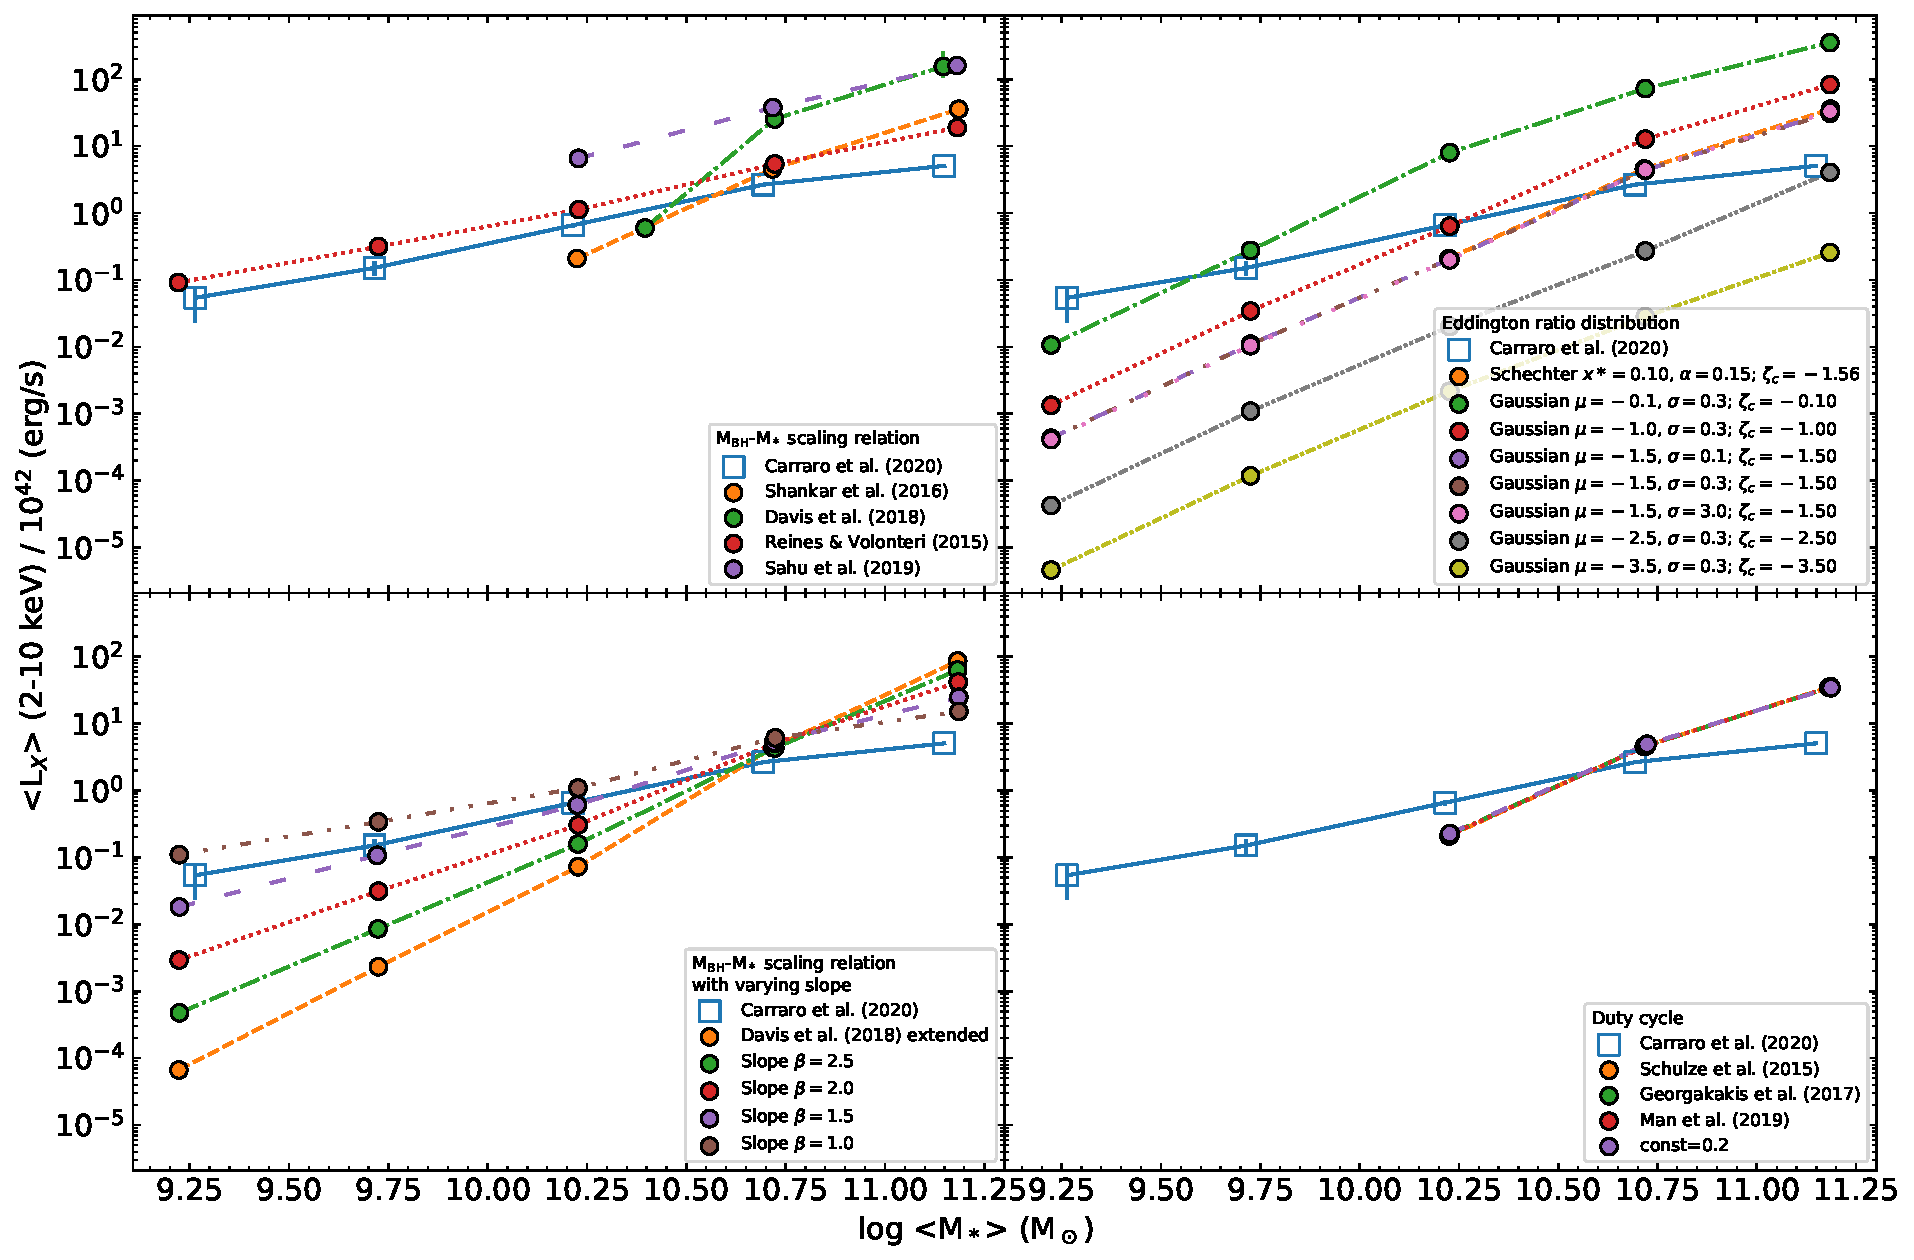
\includegraphics[width=\textwidth]{Figs/Chapter3/fig2_z1.0.pdf}
  \caption{A gallery of L$_{\rm X}-{\rm M}_*$ relations obtained by varying one of the input relations at a time. The relation that varies in each subplot is reported in the legend. 
  %Broken lines are added to the plot to guide the reader. All data-points are at $z=1$.
  Results from COSMOS data at $z=1$ from  \citet{2020A&A...642A..65C} (blue squares) are included in all plots for comparison.
  %All data-points are at $z=1$.
  Top left: L$_{\rm X}-{\rm M}_*$ relation obtained by changing the M$_{\rm BH}-{\rm M}_*$ scaling relation.
  Top right: L$_{\rm X}-{\rm M}_*$ relation obtained by changing the Eddington ratio distribution function. We use a Schechter function and Gaussian function in $\log(\lambda)$ with varying mean $\mu$ and standard deviation $\sigma$ values.
  Bottom left: L$_{\rm X}-{\rm M}_*$ relation obtained with a toy M$_{\rm BH}-{\rm M}_*$ scaling relation where we change the logarithmic slope $\beta$ of the relation $\log {\rm M}_{\rm BH} = \alpha + \beta \log {\rm M}_*$.
  Bottom right: L$_{\rm X}-{\rm M}_*$ relation obtained by changing the duty cycle method. %The slope and normalisation of the M$_{\rm BH}-{\rm M}_*$ relation as well as the mean/characteristic Eddington ratio, can all play a role in shaping the observed L$_{\rm X}-{\rm M}_*$ relation.
  }
    \label{fig:LX_M}
\end{center}
\end{figure*}

Following the procedure described above we generate diverse galaxy mock catalogs with distinct choices of the input scaling relations, duty cycles, and P($\lambda$) distributions. 
%used in the model. In particular we choose a model as a reference for all model variations. Unless differently specified, the reference relations used to generate a galaxy catalog are: %\citet{2008ApJ...688..709T} for halo mass function,  \citet{2019MNRAS.483.2506G} for halo central galaxy, 
%\citet{2016MNRAS.460.3119S} intrinsic for M$_{\rm BH}-{\rm M}_*$ scaling relation, a Schechter function as Eddington ratio distribution with a low end slope $\alpha=1.6$ and $\log(\lambda^*)=-0.8$, a modified version of \citet{2012MNRAS.425..623L} as in \citet{2020A&A...642A..65C} as bolometric correction, and \citet{2010A&A...516A..87S,2015MNRAS.447.2085S} as duty cycle.
We then divide each AGN mock catalog in bins of stellar mass, and perform 500 bootstraps on the SFR and X-ray luminosity out of which we extract the median 
%on each loop and we plot the median of the distribution 
and the 5th and 95th percentiles, following the same procedure applied to the comparison observational sample from \citet{2020A&A...642A..65C}. 
%We then compare the mocks to the data by 
%properties of the AGN mock catalogs to the observational results from  \citet{2020A&A...642A..65C} we bin the mock catalogs in the same mass bins, and perform 500 bootstraps on the SFR and X-ray luminosity out of which we extract the median on each loop and we plot the median of the distribution and the 5th and 95th percentiles as error bars, just like for the observational data.

\begin{figure*}
%%%%%\vspace{8cm}
\begin{center}
  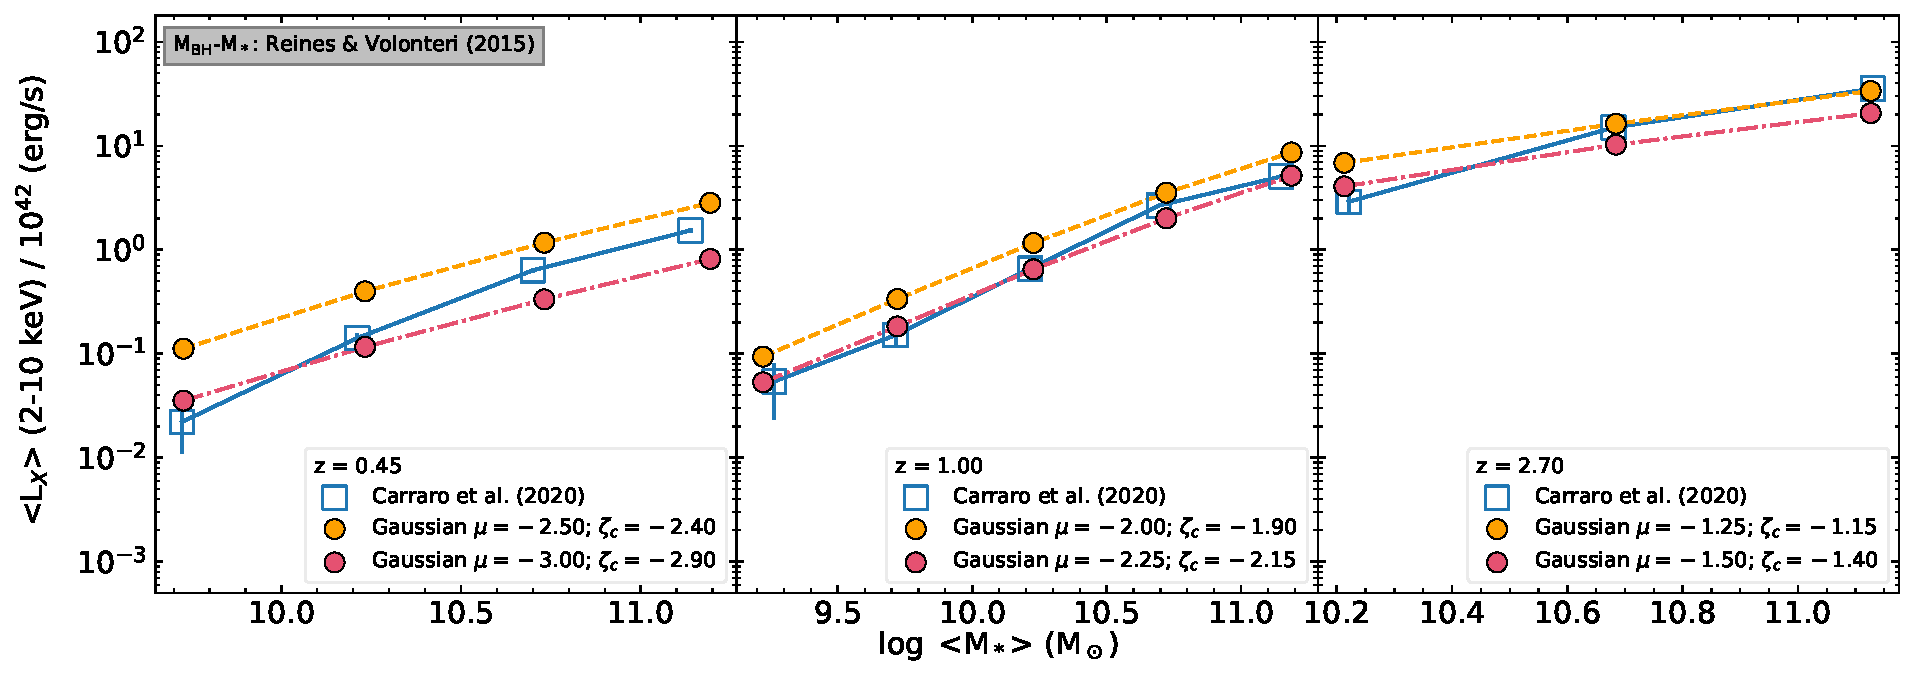
\includegraphics[width=\textwidth]{Figs/Chapter3/fig3.pdf}
  \caption{The L$_{\rm X}-{\rm M}_*$ relations at $z=0.45$ (left panels), $z=1.0$ (central panels) and $z=2.7$ (right panels) obtained by assuming a M$_{\rm BH}-{\rm M}_*$ scaling relation from \citet{2015ApJ...813...82R} and a Gaussian in $\log (\lambda)$ with standard deviation $\sigma=0.3$~dex. We vary the Eddington ratio distribution in order to reproduce the observational results from  \citet{2020A&A...642A..65C}.}

    \label{fig:LX_M_redshift}
\end{center}
\end{figure*}

\section{Results}\label{sec:results}
%\subsection{The L$_{\rm X}-{\rm SFR}$ relation}
%In Figure~\ref{fig:SFR_LX} we compare the L$_{\rm X}-{\rm SFR}$ relation from  \citet{2020A&A...642A..65C} with the same relation obtained from mock catalogues generated at $z=1$ by varying the M$_{\rm BH}-{\rm M}_*$ scaling relation.

%The mock catalogues show that there is always a relation between L$_{\rm X}-{\rm SFR}$ in which more massive galaxies are both more star forming, as by construction, and also more X-ray luminous. The  normalisation and slope of the relations vary with scaling relation. In particular the L$_{\rm X}-{\rm SFR}$ relation from using \citet{2015ApJ...813...82R} and \citet{2019ApJ...876..155S} have higher normalizations than the observations but a similar slope to the observed data-points, while \citet{2016MNRAS.460.3119S} and \citet{2018ApJ...869..113D} have a steeper slope.

%It is worth emphasising that the SFR and L$_{\rm X}$ in the mock catalogues are obtained in completely independent ways so that the relations we find in the mock catalogues is born naturally from the introduction in the code of the dependence on stellar mass of the SFR and the M$_{\rm BH}$.

\subsection{The effect of the model's inputs on the L$_{\rm X}-{\rm M}_*$ relation} \label{ssec:Fig2}

%To better understand what relations rule the L$_{\rm X}$ dependence on stellar mass, we ran simulations by changing one of the input relations in the model at a time. 
To pin down the input parameters that mostly control the L$_{\rm X}-{\rm M}_*$ relation, we explore in Figure~\ref{fig:LX_M} how the relation % In Figure~\ref{fig:LX_M} we show the L$_{\rm X}-{\rm M}_*$ relation 
 varies by changing, in turn, the M$_{\rm BH}-{\rm M}_*$ scaling relation, the Eddington ratio distribution, the duty cycle and
 a toy model $\log {\rm M}_{\rm BH} = \alpha + \beta \log {\rm M}_*$ with normalization as given by \citet{2018ApJ...869..113D},
 and varying slope, as labeled. 
 %finally we show a toy model in which we considered the \citet{2018ApJ...869..113D} scaling relation with a shape $\log {\rm M}_{\rm BH} = \alpha + \beta \log {\rm M}_*$ with $\beta=3.05$, extended it to all mass bins in consideration, and varied its slope. 
All the mocks are generated at $z=1$, though the results are applicable at all redshifts, as further discussed below.
In this Figure we adopt, unless differently specified, a Schechter Eddington ratio distribution with a knee $\lambda*=0.1$ and a faint end slope $\alpha=0.15$, as it best reproduces the AGN X-ray luminosity function (XLF) at $z=1$ in our mock catalogs.
 
From the top-left and bottom-left plots of Fig.~\ref{fig:LX_M} we can see that there is a direct proportionality between the slope of the  M$_{\rm BH}-{\rm M}_*$ scaling relation and the slope of the L$_{\rm X}-{\rm M}_*$ relation: a shallower slope in the M$_{\rm BH}-{\rm M}_*$ scaling relation will result in a shallower L$_{\rm X}-{\rm M}_*$ relation, and vice versa. Our data are at face value consistent with a slope $\beta\approx 1$ in the M$_{\rm BH}-{\rm M}_*$ relation. 
%\textbf{These scaling relations were calibrated on local galaxy samples selected in different ways, such as samples of broad line AGN \citep{2015ApJ...813...82R}, and late and early type galaxies with dynamically measured masses \citep[respectively]{2018ApJ...869..113D,2019ApJ...876..155S}. Our galaxies are better represented by a slope that is typical of broad line AGN, like \citeauthor{2015ApJ...813...82R}'s, but the fact that this is a sample of star forming galaxies should not confuse the reader, since as we will see, the best explanation for our data is likely to be an ${\rm M}_*$ dependent Eddington ratio distribution, coupled with a steeper M$_{\rm BH}-{\rm M}_*$ scaling relation.}

The Eddington ratio (top-right panel), in turn, plays a role in determining the normalization of the L$_{\rm X}-{\rm M}_*$ relation. We can see that the Schechter distribution we assumed, with a $\zeta_c\approx-1.5$ returns the same relation as a Gaussian with $\zeta_c=\mu=-1.5$, independently of its $\sigma$. This independence on the shape of the input Eddington ratio distribution is expected as the mean X-ray luminosity at fixed stellar mass only depends on the mean/characteristic Eddington ratio $\zeta_c$ of the active galaxies at that mass.  
%We decide to assume a Gaussian Eddington ratio distribution in $\log(\lambda)$ as it is completely equivalent and makes it easy to define the $\zeta_c$ of the distribution.
%Furthermore, as we tested, the choice of a Gaussian Eddington ratio distribution is completely equivalent to a Schechter distribution with the same $\zeta_c$, in that they return the same L$_{\rm X}-{\rm M}_*$ relation.

%Finally, if we consider the dependence on the duty cycle in the bottom-right panel, we can see that there is no difference in the L$_{\rm X}-{\rm M}_*$ relations of the different AGN mock catalogues, i.e. the duty cycle plays no role in determining the normalisation and slope of the L$_{\rm X}-{\rm M}_*$ relation. This is because the duty cycle only determines the amount of active galaxies.

The bottom-right panel of Fig.~\ref{fig:LX_M} confirms that the L$_{\rm X}-{\rm M}_*$ relation is independent of the shape of the input duty cycle, i.e. of the fraction of active sources as a function of black hole and/or stellar mass. The mean X-ray luminosity will be mostly controlled by the rate at which galaxies of a given black hole/stellar mass are accreting and not by how many galaxies are active at any given time. 
%The duty cycle does not play any role in determining the normalisation or slope of the L$_{\rm X}-{\rm M}_*$ relation. %This is because the duty cycle only determines the amount of active galaxies.

It is clear from Fig.~\ref{fig:LX_M} that the slope and normalization of the input M$_{\rm BH}-{\rm M}_*$ relation, as well as the input $\zeta_c$, all play a significant, and in fact degenerate, role in shaping the L$_{\rm X}-{\rm M}_*$ relation. A flatter slope in the M$_{\rm BH}-{\rm M}_*$ relation or a mass-dependent $\zeta_c$, progressively decreasing at larger masses, could both produce a flatter slope in the L$_{\rm X}-{\rm M}_*$ relation. A decreasing $\zeta_c$ with increasing M$_{\rm BH}$ or ${\rm M}_*$  could indeed reconcile the \citet{2020A&A...642A..65C} observational results with a steeper 
M$_{\rm BH}-{\rm M}_*$ relation as calibrated in the local Universe \citep[e.g.,][]{2016MNRAS.460.3119S,2018ApJ...869..113D}. 

%If we assume, for the sake of the exercise, the \citet{2016MNRAS.460.3119S} scaling relation to be valid down to $10^9M_\odot$, we can see that the normalisation of the L$_{\rm X}-{\rm M}_*$ relation decreases by decreasing the mean value $\mu$. The standard deviation is degenerate with $\mu$, for low values of $\sigma$ we will have $\zeta_c=\mu$ while by increasing $\sigma$ we will start to shift $\zeta_c$ more and more. When very close to the edge values of the $\lambda$ range, large $\sigma$ values can change the $\zeta_c$ of the distribution. This plot shows that the data is compatible with an M$_*$ dependent Eddington ratio distribution with a $\mu$ that increases with decreasing M$_*$ or, as already mentioned, with a combination of a scaling relation with a slope $\beta\sim1$ and a suitable normalisation, i.e. an Eddington ratio distribution with a suitable $\zeta_c$.

The results reported in Fig.~\ref{fig:LX_M} point to the L$_{\rm X}-{\rm M}_*$ relation as a powerful tool to constrain the mean rate of accretion of black holes $\zeta_c$ as a function of time and black hole mass in ways independent of the duty cycle. 
The AGN XLF is in fact a convolution of the underlying black hole mass function, which mostly depends on the BH-galaxy scaling relations \citep[e.g.,][]{Salucci99}, the fraction of active black holes as a function of black hole mass (the duty cycle), and the normalized Eddington ratio distribution \citep[see, e.g.,][and references therein]{Shankar13Acc}. Thus, knowledge of the AGN XLF and of the characteristic $\zeta_c$ could shed light on the duty cycle if a robust estimate of the underlying black hole-galaxy scaling relation is available from, e.g., AGN clustering measurements \citep[see discussion in][]{ShankarNat}.

%We would like to point out that our results do not depend on the particular choice of the duty cycle and on whether the mock catalogues are able to reproduce the AGN X-ray luminosity function (XLF). In fact, since the AGN XLF is degenerate with the duty cycle and the Eddington ratio distribution for a fixed M$_{\rm BH}-{\rm M}_*$ relation, we can always reproduce the AGN XLF by adopting a suitable duty cycle without affecting our results \citep{Shankar13Acc}.

%These results, and the ones in Section~\ref{subsec:SFQSB} are redshift independent since the M$_{\rm BH}-{\rm M}_*$ scaling relation is redshift independent and the effect of the model input parameters in question will be qualitatively the same at any redshift.

\subsection{Reproducing the ${\rm L}_{\rm X}-{\rm M}_*$ relation through cosmic time}

In this Section we extend the comparison to data on the L$_{\rm X}-{\rm M}_*$ relation at different redshifts. The data point to a steady decrease of the mean ${\rm L}_{\rm X}$ luminosity with cosmic time at fixed host galaxy stellar mass. As discussed above, this decreasing trend could be interpreted either as a progressive decline in the normalization of the M$_{\rm BH}-{\rm M}_*$ relation and/or in the characteristic $\zeta_c$. The latest data suggest a rather weak evolution in the M$_{\rm BH}-{\rm M}_*$ relation up to at least $z\sim 2.5$ \citep[e.g.,][]{Suh20,Shankar20MNRAS} thus favoring, in our approach, a steady decrease in $\zeta_c$, which would also be in line with independent observations \citep[]{Kollmeier06} and continuity equation models \citep[][]{Shankar13Acc,Aversa15}.

%We now want to study the evolution of the characteristic Eddington ratio. In order to simplify this, and based on our results from Fig.~\ref{fig:LX_M}, we choose to use the scaling relation that return the closest slope to our data and look for a suitable Eddington ratio distribution that returns a mock catalogue that reproduces the same normalisation as the data as well.
%Based on our results from Fig.~\ref{fig:LX_M} we reproduced the observed L$_{\rm X}-{\rm M}_*$ relation by combining the scaling relations that return the closest slope to our data to a suitable Eddington ratio distribution in order to return a mock catalog that reproduces the same normalisation as the data as well.
In Figure~\ref{fig:LX_M_redshift} we show the L$_{\rm X}-{\rm M}_*$ relation for mock catalogs at $z=0.45,1.0,2.7$ (left, central and right panels respectively), generated by assuming as a reference the \citet{2015ApJ...813...82R} M$_{\rm BH}-{\rm M}_*$ relation, which naturally generates a slope in the L$_{\rm X}-{\rm M}_*$ relation consistent with our data. 
%In all panels we also report our observational data at the same redshifts. 
We explore a range of Gaussian Eddington ratio distributions in $\log(\lambda)$ as in Sec.~\ref{ssec:Fig2}, with a fixed standard deviation of $\log \sigma=0.3$ dex and, at each redshift, report as a reference only three mock catalogs (colored circles) relatively close to the observed data (blue squares). We find that to reproduce the data we would need a drop of a factor of $\sim 10$ in the mean Eddington ratio from $z\sim 2.7$ to $z\sim 0.45$, which is broadly in line with some observational data and models' results \citep[see, e.g., Fig. 12 in][]{Shankar13Acc}. Our conclusions on the relatively fast drop of $\zeta_c$ with time are of course independent of the normalization and/or slope of the input M$_{\rm BH}-{\rm M}_*$ relation, as long as the latter remains roughly constant with redshift. 
%We remind the reader that, based on our results on Fig.~\ref{fig:LX_M}, bottom left panel, these relations are independent of the choice of duty cycle.
%{\bf The choice of an M$_{\rm BH}-{\rm M}_*$ scaling relation with slope of $\sim1$ doesn't mean that we are excluding compatibility with a steeper relation as found in many studies \citep{2019ApJ...885L..36D, 2019MNRAS.484.4360A, 2020A&A...642A..65C}, but it is the simplest choice for this section, since using a steeper relation would require adding an M$_*$ dependence on the $\zeta_c$.}

%The plots show that at fixed M$_{\rm BH}-{\rm M}_*$ scaling relation, the value of $\zeta_c$ that better reproduces the data decreases with redshift. The resulting L$_{\rm X}-{\rm M}_*$ relation will also scale with the normalisation of the input M$_{\rm BH}-{\rm M}_*$ scaling relation, therefore mocks generated with \citet{2019ApJ...876..155S}, which returns a higher normalisation (see Fig.~\ref{fig:LX_M}, top-left panel), will need a lower $\mu=\zeta_c$ of about a factor $\sim3$ to be compatible with the data-points, which would in turn require a significantly higher duty cycle in order to reproduce the AGN XLF.
%Furthermore, at each given redshift, we see that the mocks compatible with the observed data and generated with \citet{2015ApJ...813...82R}'s relation have a higher $\zeta_c$ than those generated with \citet{2019ApJ...876..155S}, which is more in line with previous literature {\bf (e.g. ?)}.
%\textbf{hickox+09,Kauffman\&coso09.}


\begin{figure*}
%%%%%\vspace{8cm}
\begin{center}
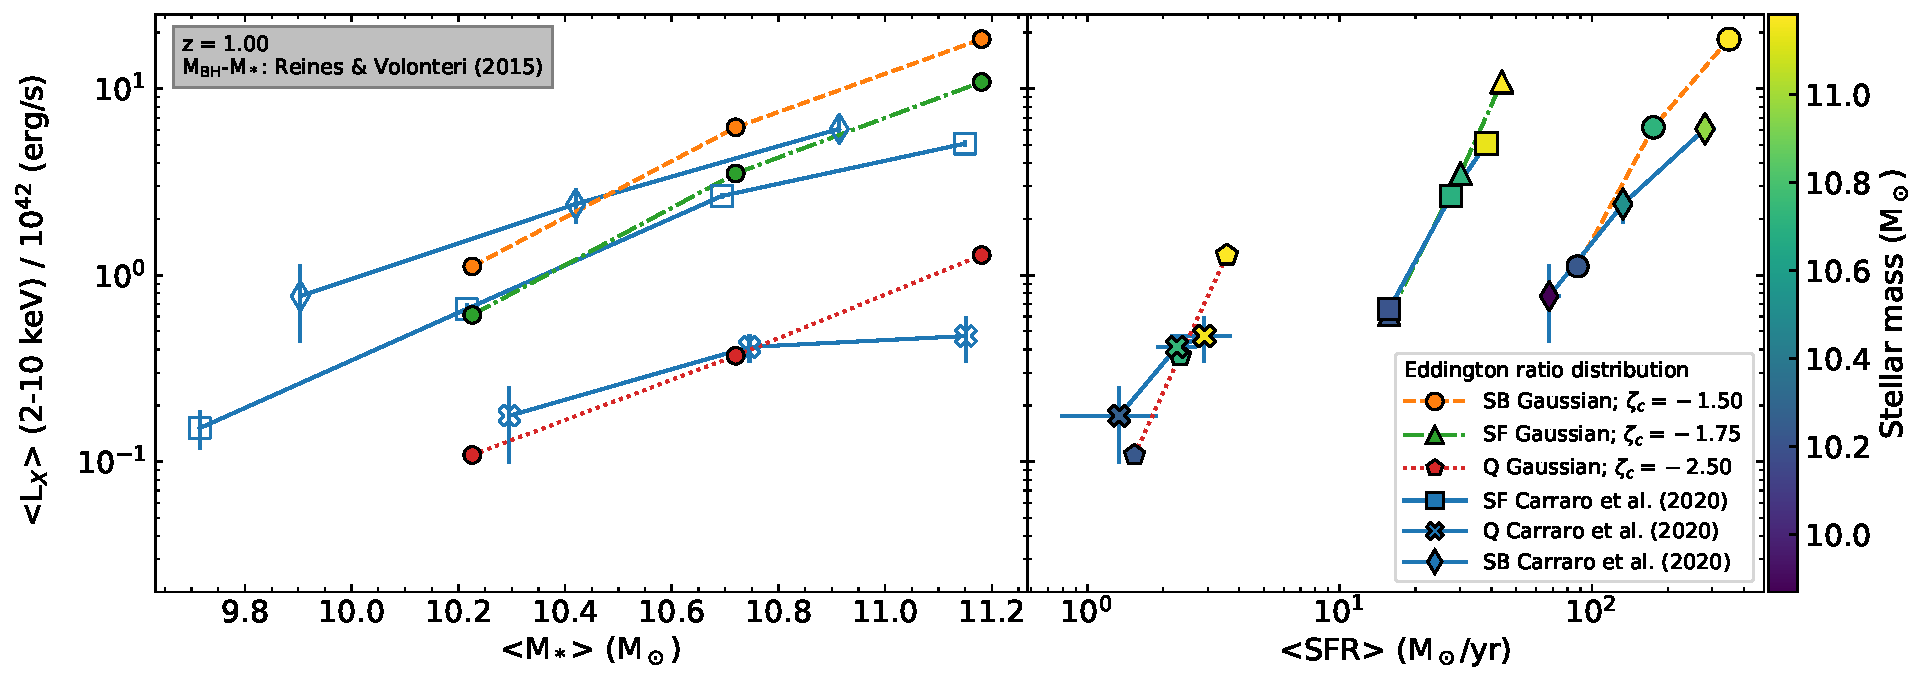
\includegraphics[width=\textwidth]{Figs/Chapter3/fig4.pdf} 
  \caption{L$_{\rm X}$ as a function of ${\rm M}_*$ (left) and SFR (right). L$_{\rm X}$ are obtained at $z=1$ with a \citet{2015ApJ...813...82R} M$_{\rm BH}-{\rm M}_*$ scaling relation and with a Gaussian Eddington ratio distribution as shown in the legend, with a $\sigma=0.3$. In the right panel, SFRs are obtained using the fits from \citet{2020A&A...642A..65C} for star-forming (SF), quiescent (Q) and starburst (SB) galaxies, and data points are color coded according to ${\rm M}_*$. All relations are compared with results from COSMOS data from \citet{2020A&A...642A..65C}.}
    \label{fig:SFQSB}
\end{center}
\end{figure*}

\subsection{Reproducing the ${\rm L}_{\rm X}-{\rm M}_*$ relation in starburst, main-sequence and quiescent galaxies} \label{subsec:SFQSB}

In this Section we focus on the dependence of the ${\rm L}_{\rm X}-{\rm M}_*$ relation on galaxy type at fixed redshift, specifically $z=1$.
%Whilst in the previous Section we probed the redshift dependence of the ${\rm L}_{\rm X}-{\rm M}_*$ relation, here we focus on its dependence on galaxy type at fixed redshift, specifically $z=1$, the mean redshift of the sample.
\citet{2020A&A...642A..65C} showed in fact that, at least at $z<2.25$, starbursts, star-forming and quiescent galaxies are characterized by distinct ${\rm L}_{\rm X}-{\rm M}_*$ relations, which are similar in slope but differ in normalization by a factor of $\sim 10$ when moving from quiescent galaxies, with the lowest average L$_{\rm X}$, to the starbursts, with the largest average L$_{\rm X}$ at fixed stellar mass. 

%The average L$_{\rm X}$ has been shown to vary depending also on the galaxy life phase so, 
In the left panel of Fig.~\ref{fig:SFQSB} we explore mocks with a constant input M$_{\rm BH}-{\rm M}_*$ relation from \citet{2015ApJ...813...82R}, and a varying $\zeta_c$ (circles, triangles, and pentagons) against the different data sets for the three types of galaxies studied by \citet{2020A&A...642A..65C} (blue diamonds, squares and crosses for starbursts, star-forming, and quiescent galaxies respectively). Reproducing the steep increase of $\sim 10$ in mean ${\rm L}_{\rm X}$ requires, as expected, an equal overall increase in $\zeta_c$. Interestingly, the observed ${\rm L}_{\rm X}-{\rm M}_*$ relation is not a simple power law but tends to show a break that becomes more pronounced in more massive quiescent galaxies of mass $\log (M_*/M_{\odot}) \gtrsim 11$. In our modeling this feature could be naturally reproduced with a further decrease in $\zeta_c$ in the most massive and quiescent galaxies in our sample, which would align with the idea of downsizing, supporting the view that more massive galaxies and their central black holes have accreted their mass at a faster pace and are now in their declining phase. We note that the downsizing in $\zeta_c$ would be even more pronounced if steeper M$_{\rm BH}-{\rm M}_*$ relations were adopted in input. The right panel of Fig.~\ref{fig:SFQSB} shows that our chosen values of $\zeta_c$ that match the ${\rm L}_{\rm X}-{\rm M}_*$ relation for each galaxy type also reproduce, at the same time, their respective ${\rm L}_{\rm X}-{\rm SFR}$ relations, where the SFR is assigned to each galaxy type based on their observed underlying ${\rm M}_*-{\rm SFR}$ relation. 

%by varying the $\zeta_c$ that reproduce the observed L$_{\rm X}$ from \citet{2020A&A...642A..65C} for starburst and quiescent galaxies. In the left panel, we can see that the ${\rm L}_{\rm X}-{\rm M}_*$
%We now want to see how to reproduce the L$_{\rm X}$ of the observed quiescent and starburst galaxies from \citet{2020A&A...642A..65C}. In Fig.~\ref{fig:SFQSB}, left panel, we can see that the ${\rm L}_{\rm X}-{\rm M}_*$ of starburst and quiescent galaxies 
%can be reproduced by increasing and decreasing respectively, $\zeta_c$ with respect to star forming galaxies. 
%This sounds reasonable since starburst galaxies are gas rich galaxies undergoing intense episodes of star formation while quiescent galaxies have consumed most of their gas. In these two life phases it is even more apparent that a lower $\zeta_c$ is needed at high stellar masses in order to reproduce the observed data. This is a sign of downsizing, i.e. the fact that more massive galaxies have accreted their stellar and BH masses at very high redshift and have slowed down their accretions. \textbf{say something about fig.3 right panel}.

An alternative way to explain the different normalizations of starburst and quiescent galaxies in the ${\rm L}_{\rm X}-{\rm M}_*$ plane would be to adopt the same $\zeta_c$ for all galaxy types and progressively increase the normalization of the M$_{\rm BH}-{\rm M}_*$ scaling relation when moving from quiescent to starburst galaxies. %For quiescent galaxies, this would imply a lower normalisation of the scaling relation, and therefore a lower M$_{\rm BH}$ at given M$_*$, 
However, such a solution would not be favored from an evolutionary point of view as quiescent galaxies should be older galaxies with larger black holes at fixed stellar mass.
%more ``mature'' galaxies with, if anything, larger black holes at fixed stellar mass. 

All in all, the evolutionary picture that could be extracted from Fig.~\ref{fig:SFQSB} is one in which the central black hole and its host galaxy move around a similar M$_{\rm BH}-{\rm M}_*$ scaling relation throughout their lifetime. They could start from a main-sequence or even starburst, gas-rich phase, evolving at an almost constant (specific) SFR, as also proposed by theoretical models \citep[e.g.][]{2014ApJ...782...69L, Aversa15} and direct observations \citep{2020A&A...642A..65C}, and then gradually switch off their accretion and star formation due to internal gas consumption, thus gradually reducing their star formation rate and accretion onto the central black hole (right panel of Fig.~\ref{fig:SFQSB}).  
%This picture would also be
%In the evolutionary picture in which starbursts are gas rich young galaxies that evolve at an almost constant SFR, as proposed by theoretical models \citep[e.g.][]{2014ApJ...782...69L, Aversa15}, it may be thought that galaxies are born with a certain M$_{\rm BH}-{\rm M}_*$ scaling relation that is constant in time and have a decrease of $\zeta_c$ in time, as galaxies evolve to become star forming and then quiescent. This would be further supported by the mild L$_{\rm X}$ evolution of starburst galaxies shown in \citet{2020A&A...642A..65C}.

\section{Discussion and conclusions}\label{sec:disc_concl}

%In this work we took advantage of SEMs to generate mock galaxy catalogs onto which we performed a statistical study, analogous to our previous work (Carraro et al. 2020). We used semi-empirical relations to study the L$_{\rm X}-{\rm M}_*$ relation. We started from a halo mass function at a given redshift, we assign galaxies and black holes to dark matter haloes via the most up-to-date empirical stellar-halo and M$_*-{\rm M}_{\rm BH}$ relations and we assumed an SFR depending only on stellar mass and redshift. We explored a range of Eddington ratio distributions, M$_*-{\rm M}_{\rm BH}$ scaling relations and duty cycles in order to determine what drives the shape of the L$_{\rm X}-{\rm M}_*$ relation.
In this Letter we use statistical semi-empirical models to generate accurate mock catalogs of active galaxies, which we analyze in the same manner as in the comparison observational sample  \citep{2020A&A...642A..65C}. Our goal is to unveil the input parameters driving the L$_{\rm X}-{\rm M}_*$ relation. We start from a halo mass function at a given redshift, we assign galaxies and black holes to dark matter haloes via the most up-to-date empirical stellar-halo and M$_{\rm BH}-{\rm M}_*$ relations and we assume a SFR depending only on stellar mass and redshift. We explore a range of Eddington ratio distributions, M$_{\rm BH}-{\rm M}_*$ scaling relations and duty cycles.

We show that the L$_{\rm X}$-SFR or L$_{\rm X}-{\rm M}_*$ is independent of the AGN duty cycle, but strongly depends on the shape of the M$_{\rm BH}-{\rm M}_*$ scaling relation and on the characteristic Eddington ratio $\zeta_c$, linking the mean L$_{\rm X}$ with the M$_{\rm BH}$. The L$_{\rm X}-{\rm M}_*$ relation can break degeneracies among input duty cycles, Eddington ratio distributions and also BH-galaxy scaling relations, especially when the latter are coupled with AGN clustering measurements \citep{ShankarNat}, thus representing a powerful tool for cosmological models. The AGN XLF, for example, is a product of the underlying BH mass function% (which only depends on the M$_{\rm BH}-{\rm M}_*$ relation)
, the duty cycle and underlying Eddington ratio distribution.
We find that our current data on L$_{\rm X}-{\rm M}_*$ favor, at fixed $\zeta_c$, flatter M$_{\rm BH}-{\rm M}_*$ relations, or M$_*$ dependent $\zeta_c$ at fixed M$_{\rm BH}-{\rm M}_*$. An M$_*$ dependent $\zeta_c$ combined with a steeper M$_{\rm BH}-{\rm M}_*$ relations would indeed be favored by different observational studies \citep{2019ApJ...885L..36D, 2019MNRAS.484.4360A, 2020A&A...642A..65C}, continuity equation arguments \citep{Shankar13Acc,Aversa15} and population synthesis models \citep{2018MNRAS.476..436B}.
%More specifically, we find that the $\zeta_c$ is a factor of $\sim 3$ lower when adopting the \citet{2019ApJ...876..155S} relation compared to \citet{2015ApJ...813...82R}, which would in turn require a significantly higher duty cycle in order to reproduce the AGN XLF.

In our previous work  \citep[see, e.g., Fig.~3 in][]{2020A&A...642A..65C} we have shown that main-sequence and quiescent galaxies share at all probed cosmic epochs similar ratios of BHAR and SFR suggesting that the two processes are linked together throughout different galaxy phases.  
%have higher specific star formation rates than quiescent galaxies proportionally higher mean L$_{\rm X}$ at fixed M$_*$. 
In our framework, this correspondence between specific SFR and mean L$_{\rm X}$ can be viewed as an evolution in $\zeta_c$, being on average higher in more star-forming galaxies and significantly lower in quiescent galaxies, especially at higher stellar masses and at lower redshifts, in line with a scenario in which the AGN activity gradually switches off along with the SFR. This effect is visible also in starburst galaxies, though their ratio between mean BHAR and SFR tends to be, at any given epoch, a factor of a few lower, possibly due to a more restrictive limit on the accretion on to the central black hole.

%\begin{figure}[t]
%\begin{center}
%  \includegraphics[scale=0.5, angle=-90]{photo.png}
%  \caption{Here you can provide the caption.}
%    \label{and_the_label}
%  }
%\end{center}
%\end{figure}
